\documentclass{standalone} 
\PassOptionsToPackage{usenames,dvipsnames,svgnames}{xcolor}  
\usepackage{tikz}
\usetikzlibrary{arrows,positioning,automata}

\begin{document}
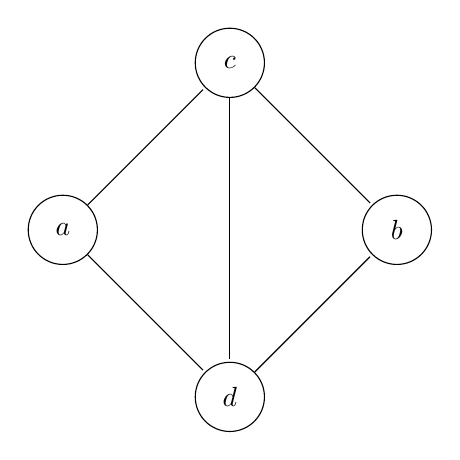
\begin{tikzpicture}[>=stealth',shorten >=1pt,node distance=3cm,on grid,initial/.style    ={}]
  \node[state]          (a)                          {$a$};
  \node[state]          (c)  [above right = of a]    {$c$};
  \node[state]          (d)  [below right = of a]    {$d$};
  \node[state]          (b)  [below right = of c]    {$b$};

  \path (a)     edge [-]                    node   {} (c);
  \path (a)     edge [-]                    node   {} (d);
  \path (c)     edge [-]                    node   {} (d);
  \path (c)     edge [-]                    node   {} (b);
  \path (d)     edge [-]                    node   {} (b);

\end{tikzpicture}
\end{document}